\chapter{The HH$\rightarrow$4b analysis}\label{ch:hh4b}

Investigating the exact shape of the Higgs potential is an interesting endeavor, as it is directly related to \ac{ewsb} and fundamental questions about the nature of the universe, as discussed in section \ref{sec:beyond_sm}. The main Higgs production modes at the \ac{lhc} are shown in Figure \ref{fig:main_production_processes} and can be understood by the fact that the Higgs boson interacts with fermions via Yukawa couplings from equation \ref{eq:yukawa_term}. Since Yukawa couplings are directly proportional to the fermion masses the Higgs boson predominantly couples to heavier particles like the top quark or the massive vector bosons. All couplings are scaled relative to their \ac{sm} values and are denoted as $\kappa_\mathrm{c} = c/c_\mathrm{sm}$. A $\kappa_\mathrm{c}$ value of 1 therforee corresponds to the \ac{sm} value for some given coupling $c$.

The first two \ac{ggf} diagrams \ref{fig:main_production_processes}(a) and \ref{fig:main_production_processes}(b) have a cross-section of $\sigma_\text{vbf HH}^\text{SM}=\qty[]{31.05}{fb}$ calculated at a center of mass energy of \qty[]{13}{TeV} at \ac{nnlo} \citep{Grazzini_2018} while the \ac{vbf} processes (c), (d) and (e) of figure \ref{fig:main_production_processes} have a production cross-section of
$\sigma_\text{vbf HH}^\text{SM}=\qty[]{1.73}{fb}$ at \ac{nnnlo} \citep{PhysRevD.98.114016}. A characteristic of the \ac{vbf} processes is that the Higgs pair products are accompanied by two additional quarks. The \ac{vbf} cross section is about \qty[]{3e4}{} times smaller than the production cross section for single Higgs $\sigma_\text{H}^\text{SM}=\qty[]{48.58}{pb}$ at the \ac{lhc} \citep{de2016arxiv} and underlines the challenge of discovering Higgs pairs in these final states.
\begin{figure}
    \centering
    \subfigure[]{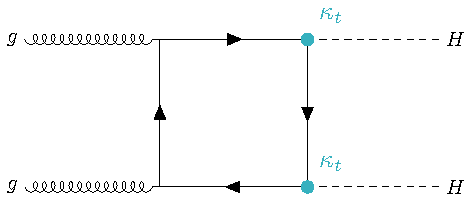
\includegraphics[width=.43\textwidth]{fig_01a}}\hspace{.06\textwidth}
    \subfigure[]{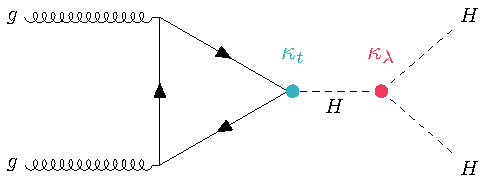
\includegraphics[width=.43\textwidth]{fig_01b}} \\
    \subfigure[]{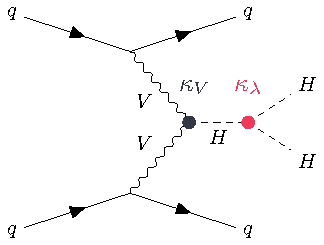
\includegraphics[width=.3\textwidth]{fig_02a}}\hspace{.01\textwidth}
    \subfigure[]{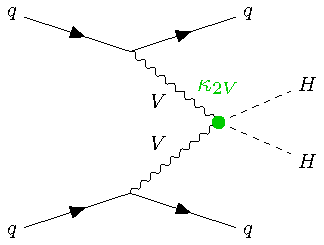
\includegraphics[width=.3\textwidth]{fig_02b}}\hspace{.01\textwidth}
    \subfigure[]{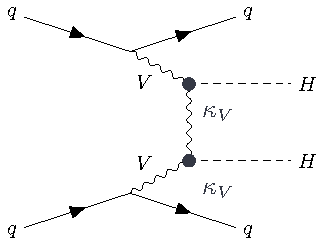
\includegraphics[width=.3\textwidth]{fig_02c}}
    \caption[]{Leading Higgs Pair production processes at the \ac{lhc}. (a), (b) shows \ac{ggf} and (c), (d), (e) \ac{vbf} processes. Adopted from \citep{aad2023search}.}
    \label{fig:main_production_processes}
\end{figure}
% higgs hat keine Ladung whatsoever cannot couple em or qcd 

\begin{figure}
    \centering
    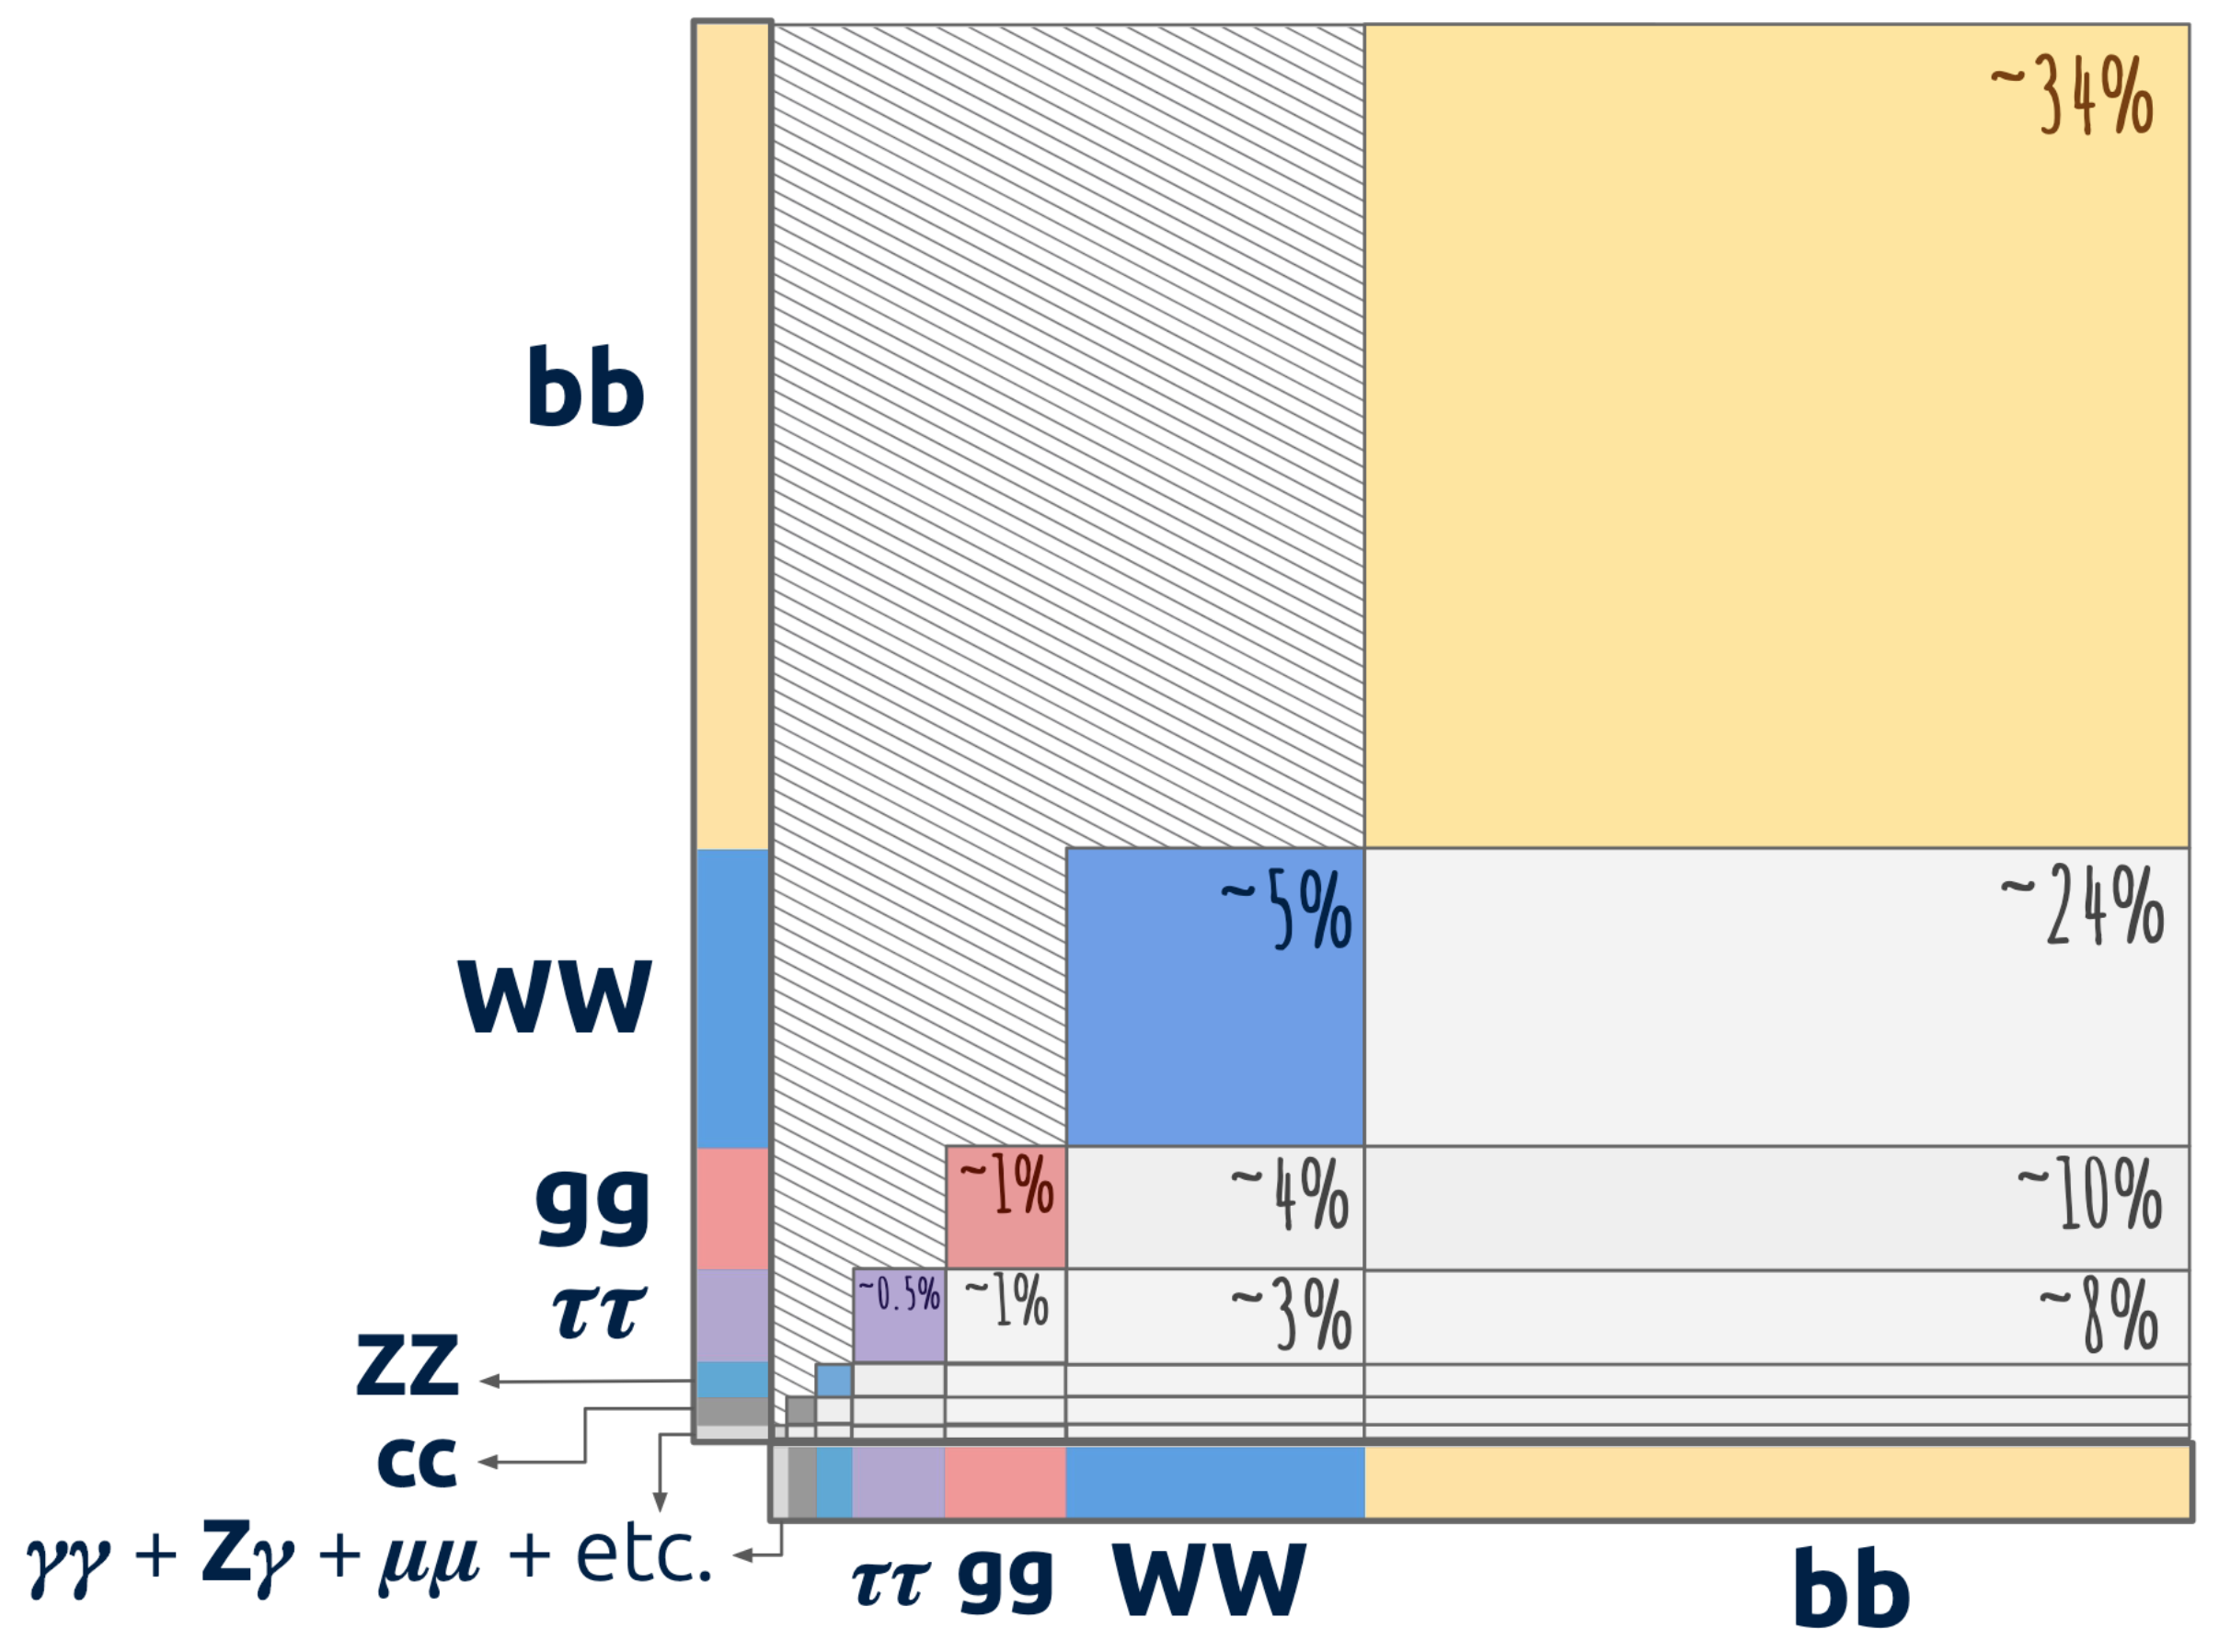
\includegraphics[width=0.7\textwidth]{branching_fraction_hh}
    \caption[]{Contributions of final states represented by area for a pair of Higgs. Adopted from \citep{ATL-COM-PHYS-2020-083}.}
    \label{fig:branching_fraction_hh}
\end{figure}
Figure \ref{fig:branching_fraction_hh} highlights that an interesting channel in the study of Higgs pair production is the final state with the largest branching fraction, which consists of four $b$ quarks and amounts to about \qty[]{34}{\percent}. Thus the \ac{sm} \ac{vbf} cross-section is calculated to correspond to the 4b branching ratio by multiplying it with $\mathcal{B}(4b)=0.3392$. This fully hadronic final state, however, presents the challenge of significant \ac{qcd} backgrounds.

This work focuses on the boosted topology of highly energetic jets which do not allow reconstruction of $b$-jets individually but rather of final states consisting of large-$R$ jets encapsulating two collimated $b$-jets inside. This approach substantially reduces \ac{qcd} backgrounds, as highly energetic jets are more likely to originate from heavy particles like $b$ quarks. Additionally, events with jets of large \pt are have a clearer signature to trigger on. While representing a comparatively clean signal, such events are rare and thus have limited statistical power. Despite other decay signatures being more suitable for the discovery of the Higgs pair production process the power of this selection lies in proving the existence of the \ktwov coupling shown in figure \ref{fig:main_production_processes}(d) to which it is directly sensitive.

The low cross-section for this process is due to the fact that diagrams (d) and (e) in Figure \ref{fig:main_production_processes} exhibit destructive interference for \ac{sm} values. Conversely, when $\ktwov$ deviates from \ac{sm} values, the production cross-section increases significantly, with $\sigma_{\ktwov=0}\approx 20\sigma_{\ktwov=1}$ and the decay products exhibit much larger transverse momentum, as illustrated in Figure \ref{fig:kappa_2v_variations_mhh}.
\begin{figure}
    \centering
    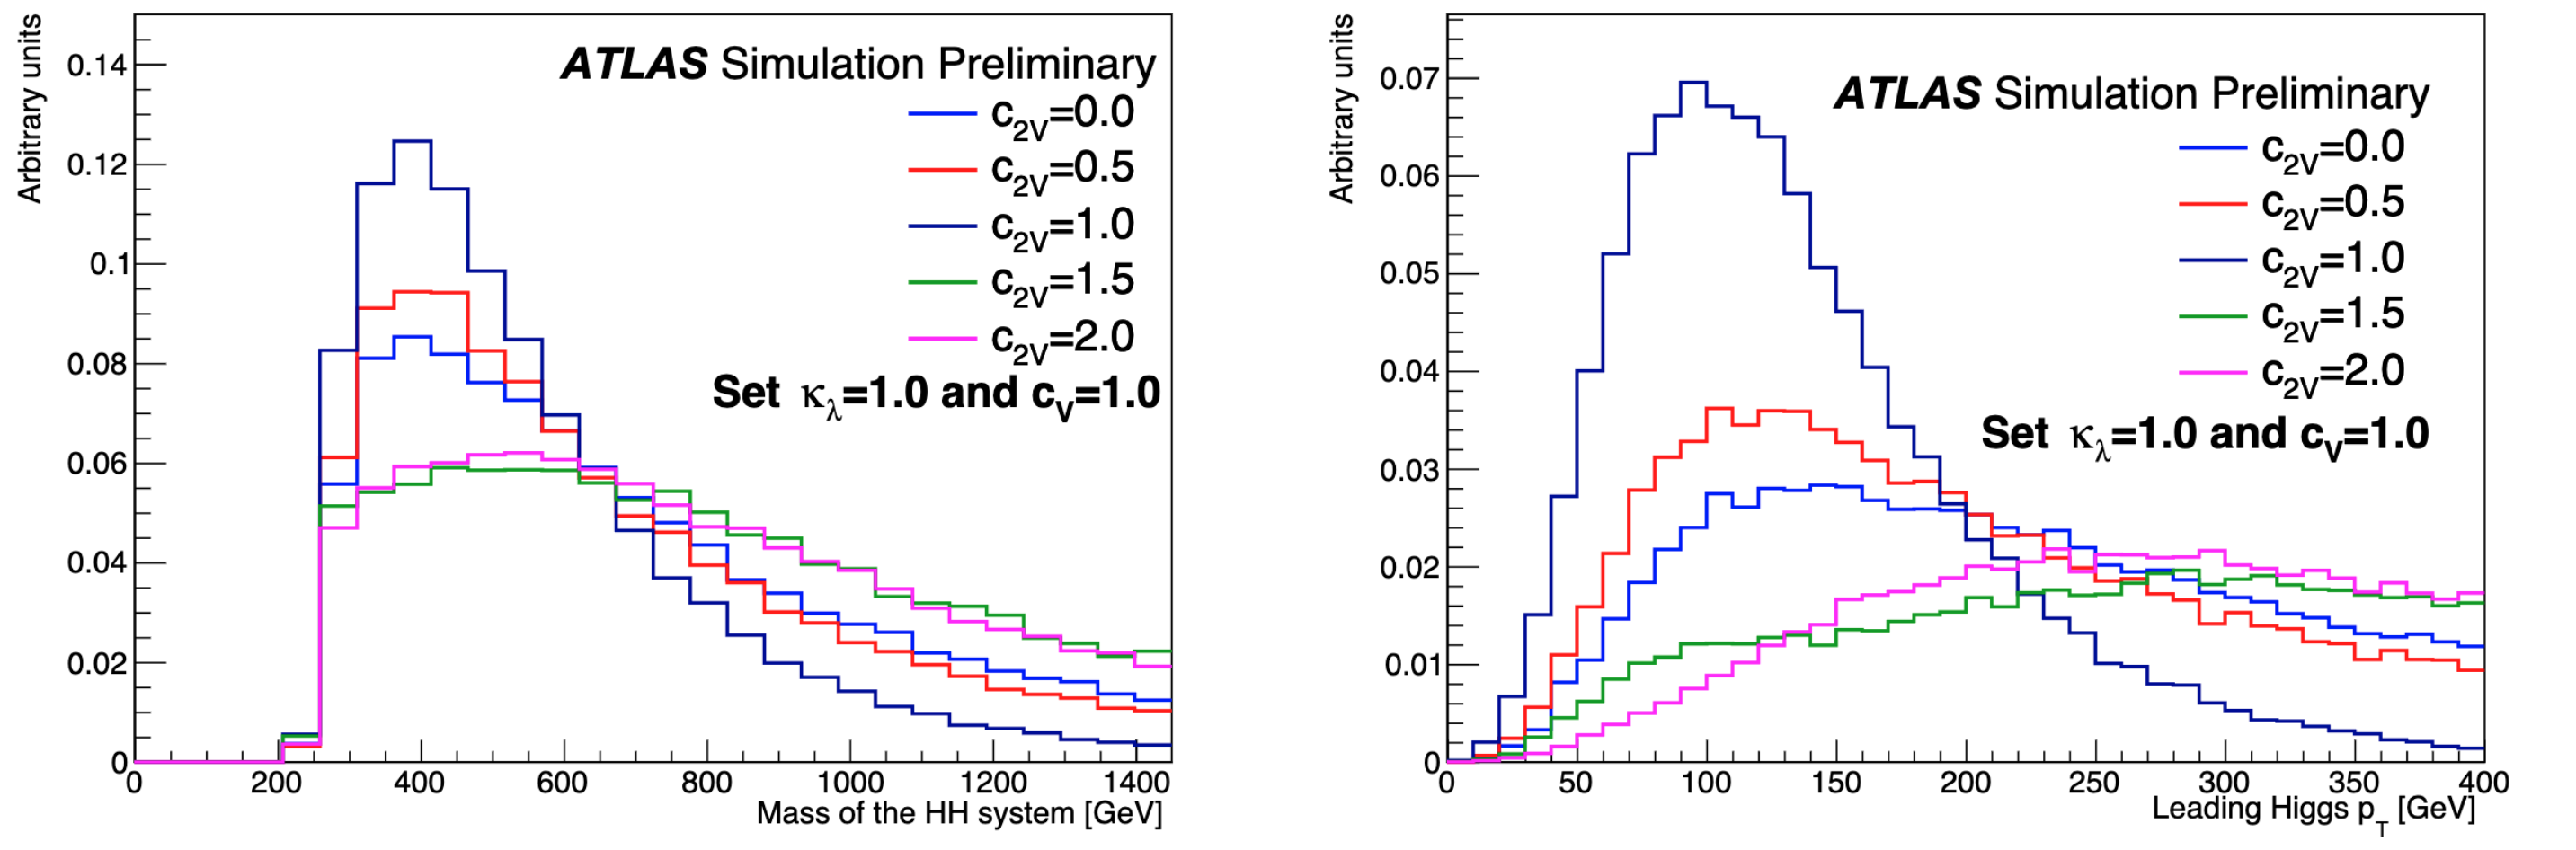
\includegraphics[width=1\textwidth]{kappa_2v_variations_mhh}
    \caption[]{Invariant mass of the Higgs pair system and the leading Higgs candidate jet \pt  reconstructed from simulation for different \ktwov. Adopted from \citep{ATL-PHYS-PUB-2019-007}.}
    \label{fig:kappa_2v_variations_mhh}
\end{figure}

\section{Data and Monte Carlo Simulation}\label{sec:mc_simulation}
This analysis uses the full run 2 data taken by \ac{atlas} between 2015 and 2018. The dataset contains \qty[]{140.1}{fb^{-1}} of data good for physics at a center of mass energy of \qty[]{13}{TeV} \citep{DAPR-2021-01}.

\ac{mc} generation in \ac{atlas} is typically done in three steps. At first at parton level the matrix element of the process of interest is stochastically simulated with \textsc{MadGraph} (v.2.7.3p3.atlas6) \citep{alwall2014automated}. The cross sectional calculation for proton-proton collisions relies on the factorization theorem \citep{halzen1984introductory} which states that contributions from partons participating in the hard scatter event can be factorized. Further partons cannot be observed individually since the approximation of the perturbation ansatz of section \ref{sec:qft} breaks down for low energy scales $\mu^2$ as described in section \ref{sec:renormalization}. This is the energy scale for which the approximation would need to hold to describe the partons inside a proton. However parton densities can be studied within \ac{qcd} using the DGLAP equations \citep{thomson2013modern}. Similar to renormalization, a scaling behavior can be derived from these equations that allows to derive an estimate of the \acp{pdf} by measuring it at some factorization scale $\mu_F^2$ in order to extrapolate it to another. Figure \ref{fig:pdf} exemplifies this for two energy scales from the \textsc{NNPDF3.0nlo} \ac{pdf} set used in this analysis.
\begin{figure}
    \centering
    \subfigure[]{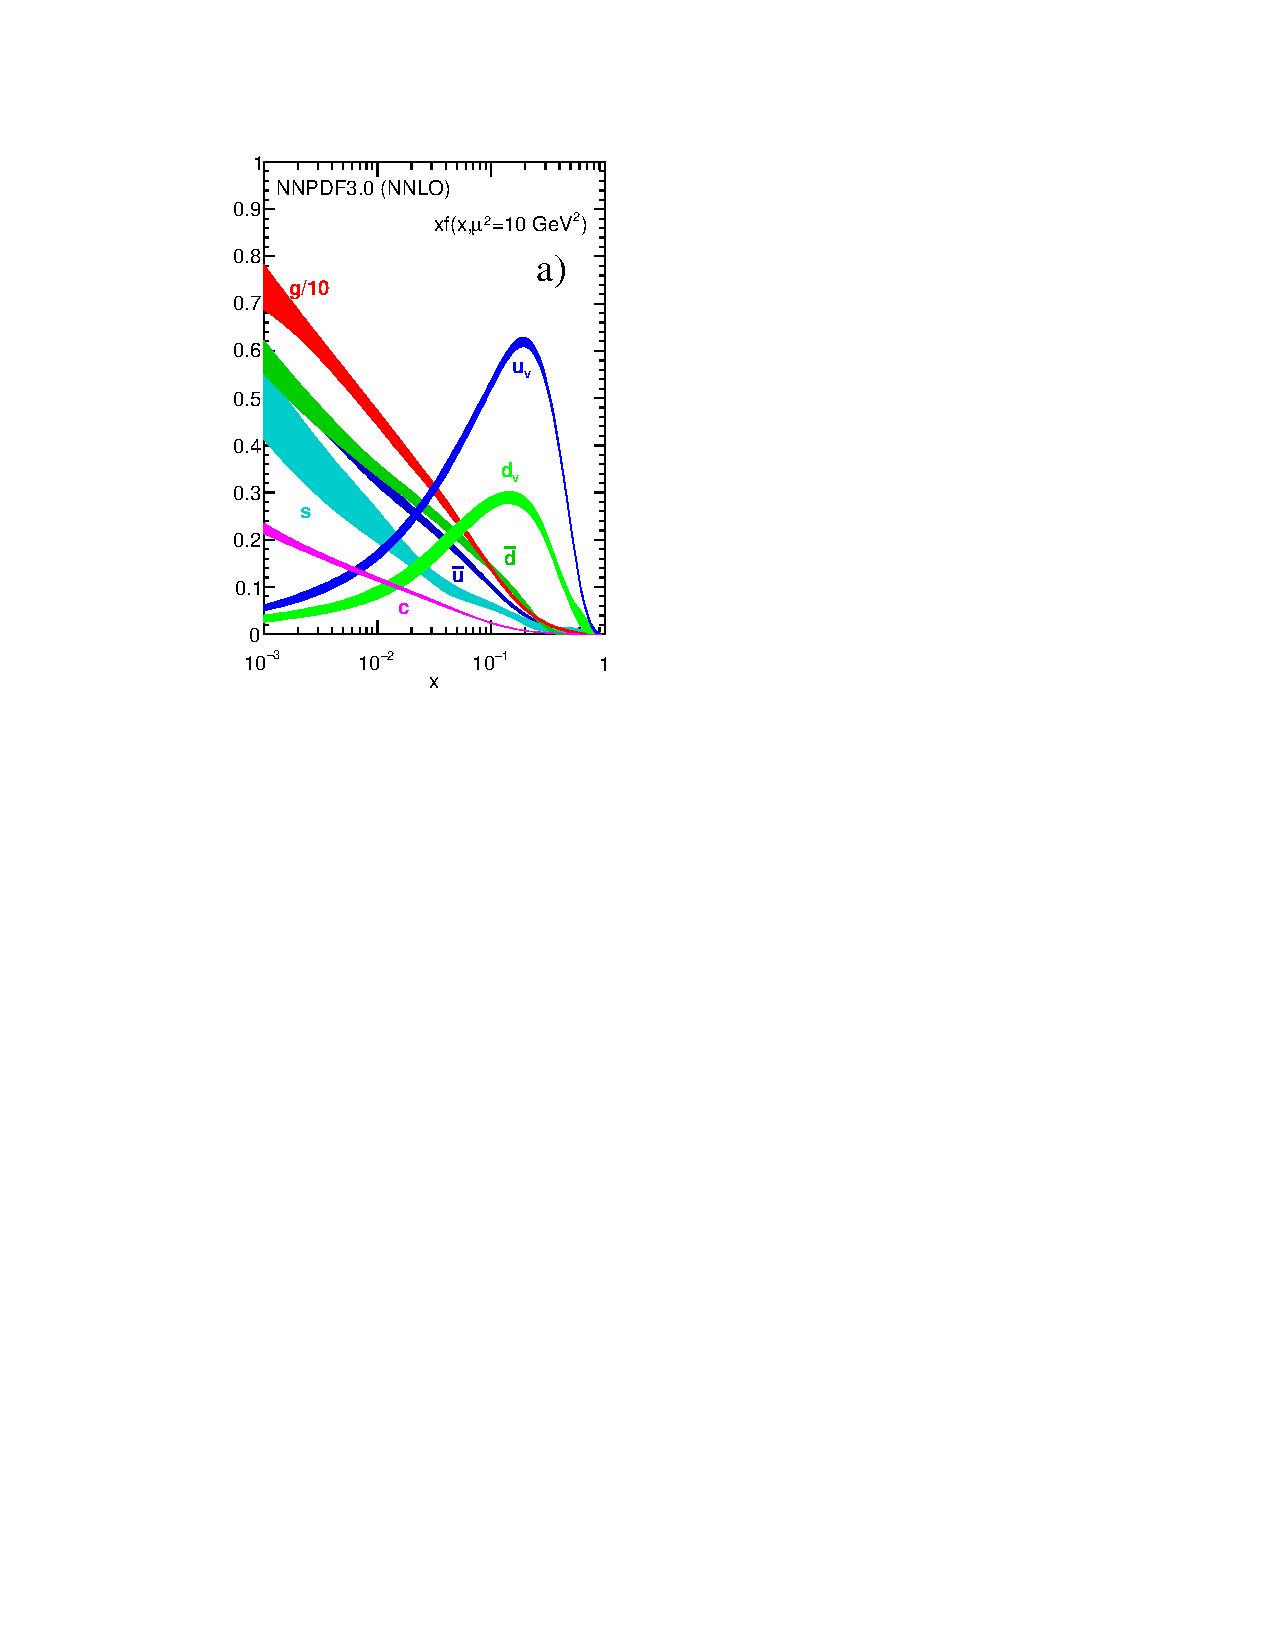
\includegraphics[width=.47\textwidth]{NNPDF-10}}
    \subfigure[]{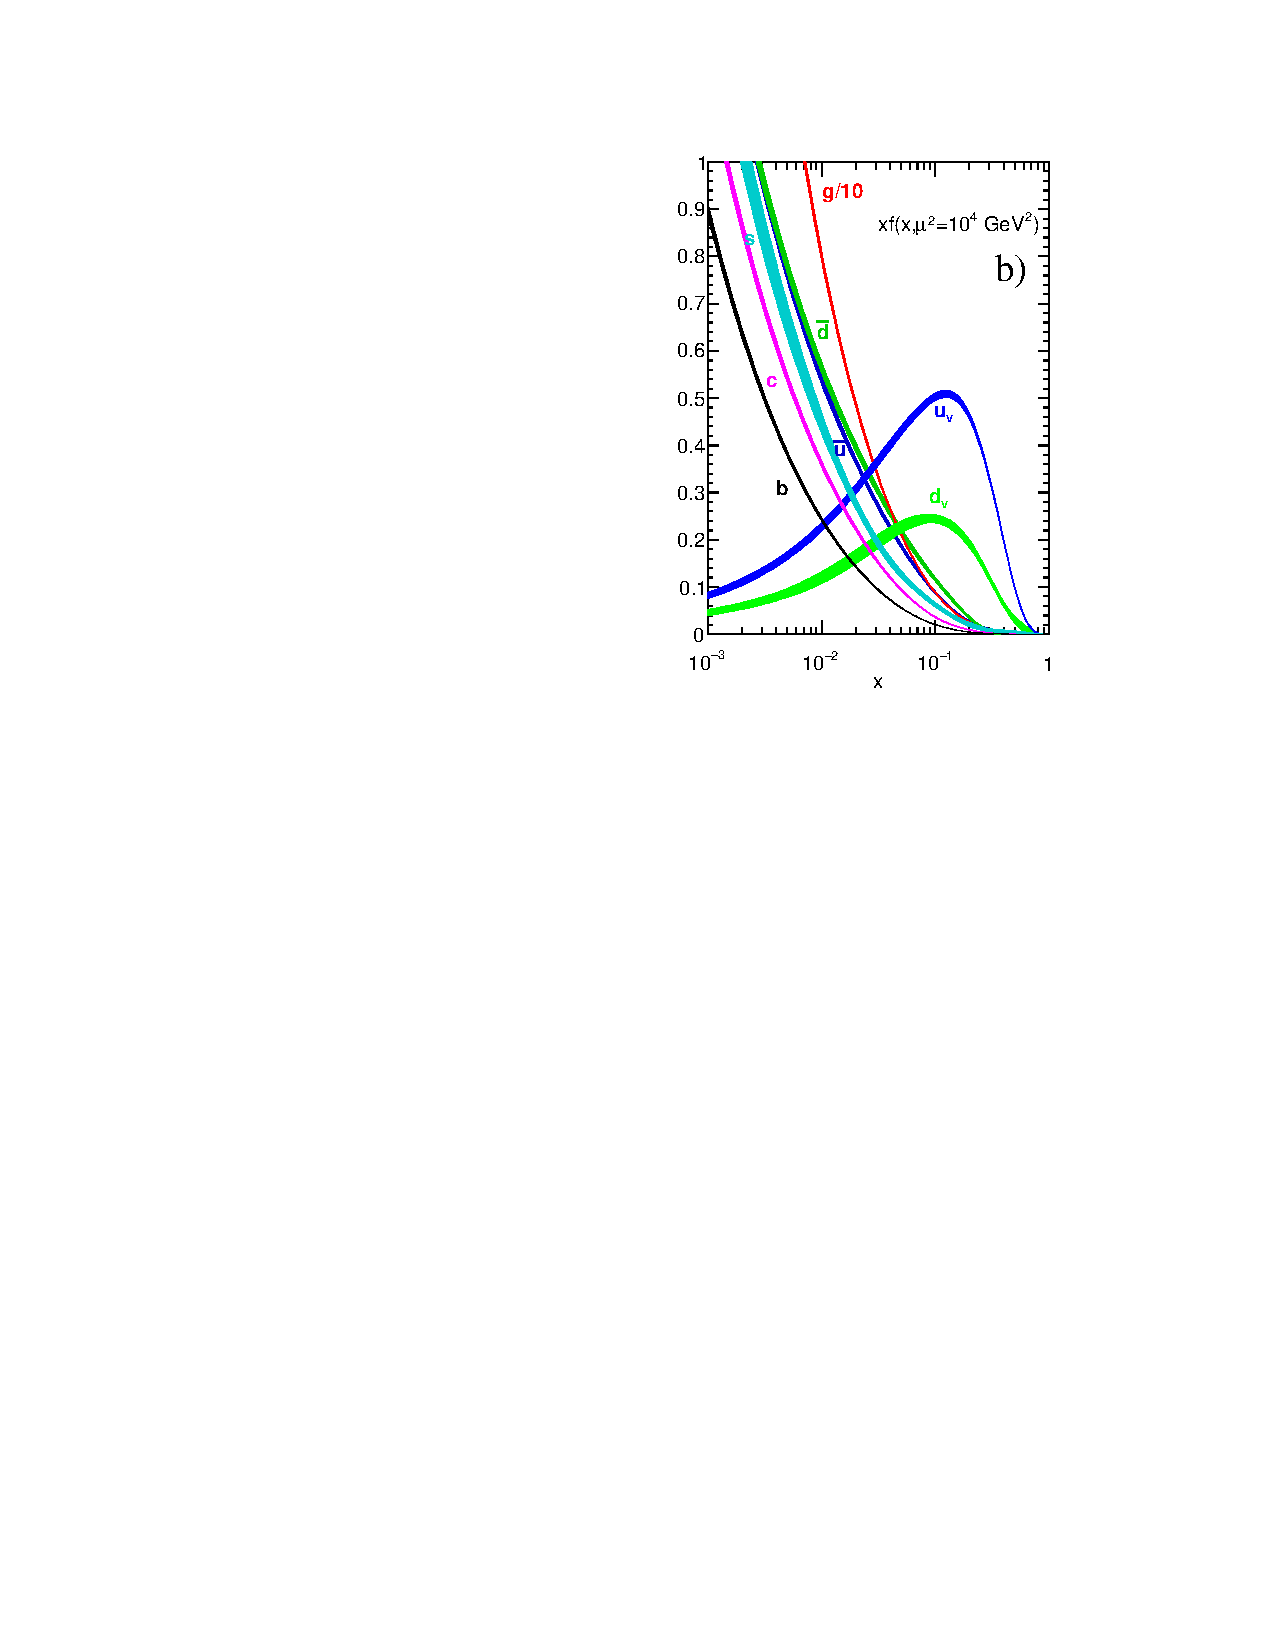
\includegraphics[width=.47\textwidth]{NNPDF-10000}}
    \caption[]{\textsc{NNPDF3.0nlo} parton distribution functions for two different factorization scales (a) $\mu_F^2=$\qty{10}{GeV}$^2$ and (b) $\mu_F^2=$\qty{10}{TeV}$^2$ against the momentum fraction $x$ of the particle. Adopted from \citep{PhysRevD.98.030001}.}
    \label{fig:pdf}
\end{figure}
Thus for hadrons $A,B$ containing partons $a,b$ and their respective \acp{pdf} $f_{a}^A$ and $f_{a}^B$, dependent on the parton's momentum fraction $x$ and factorization scale $\mu_F^2$, the cross-section of a process $A,B\rightarrow X$ reads
\begin{equation}
    \sigma_{A,B\rightarrow X} = \sum_{a,b} \int_0^1 \text{d}x_1\text{d}x_2 f_a^A(x_1,\mu_F^2) f_b^B(x_2,\mu_F^2) \hat{\sigma}_{a,b\rightarrow X}(\alpha_s(\mu_R^2),\mu_R^2).
\end{equation}
$\hat{\sigma}_{a,b\rightarrow X}$ is the perturbatively calculable part and therefore depends on the strong coupling $\alpha_S$ and renormalization scale $\mu_R^2$.

In a second step the parton shower evolution including hadronization and initial and final state radiation is simulated with \textsc{Pythia8} \citep{Sjostrand:2014zea}. Figure \ref{fig:parton_shower} illustrates this process.
\begin{figure}[]
    \centering
    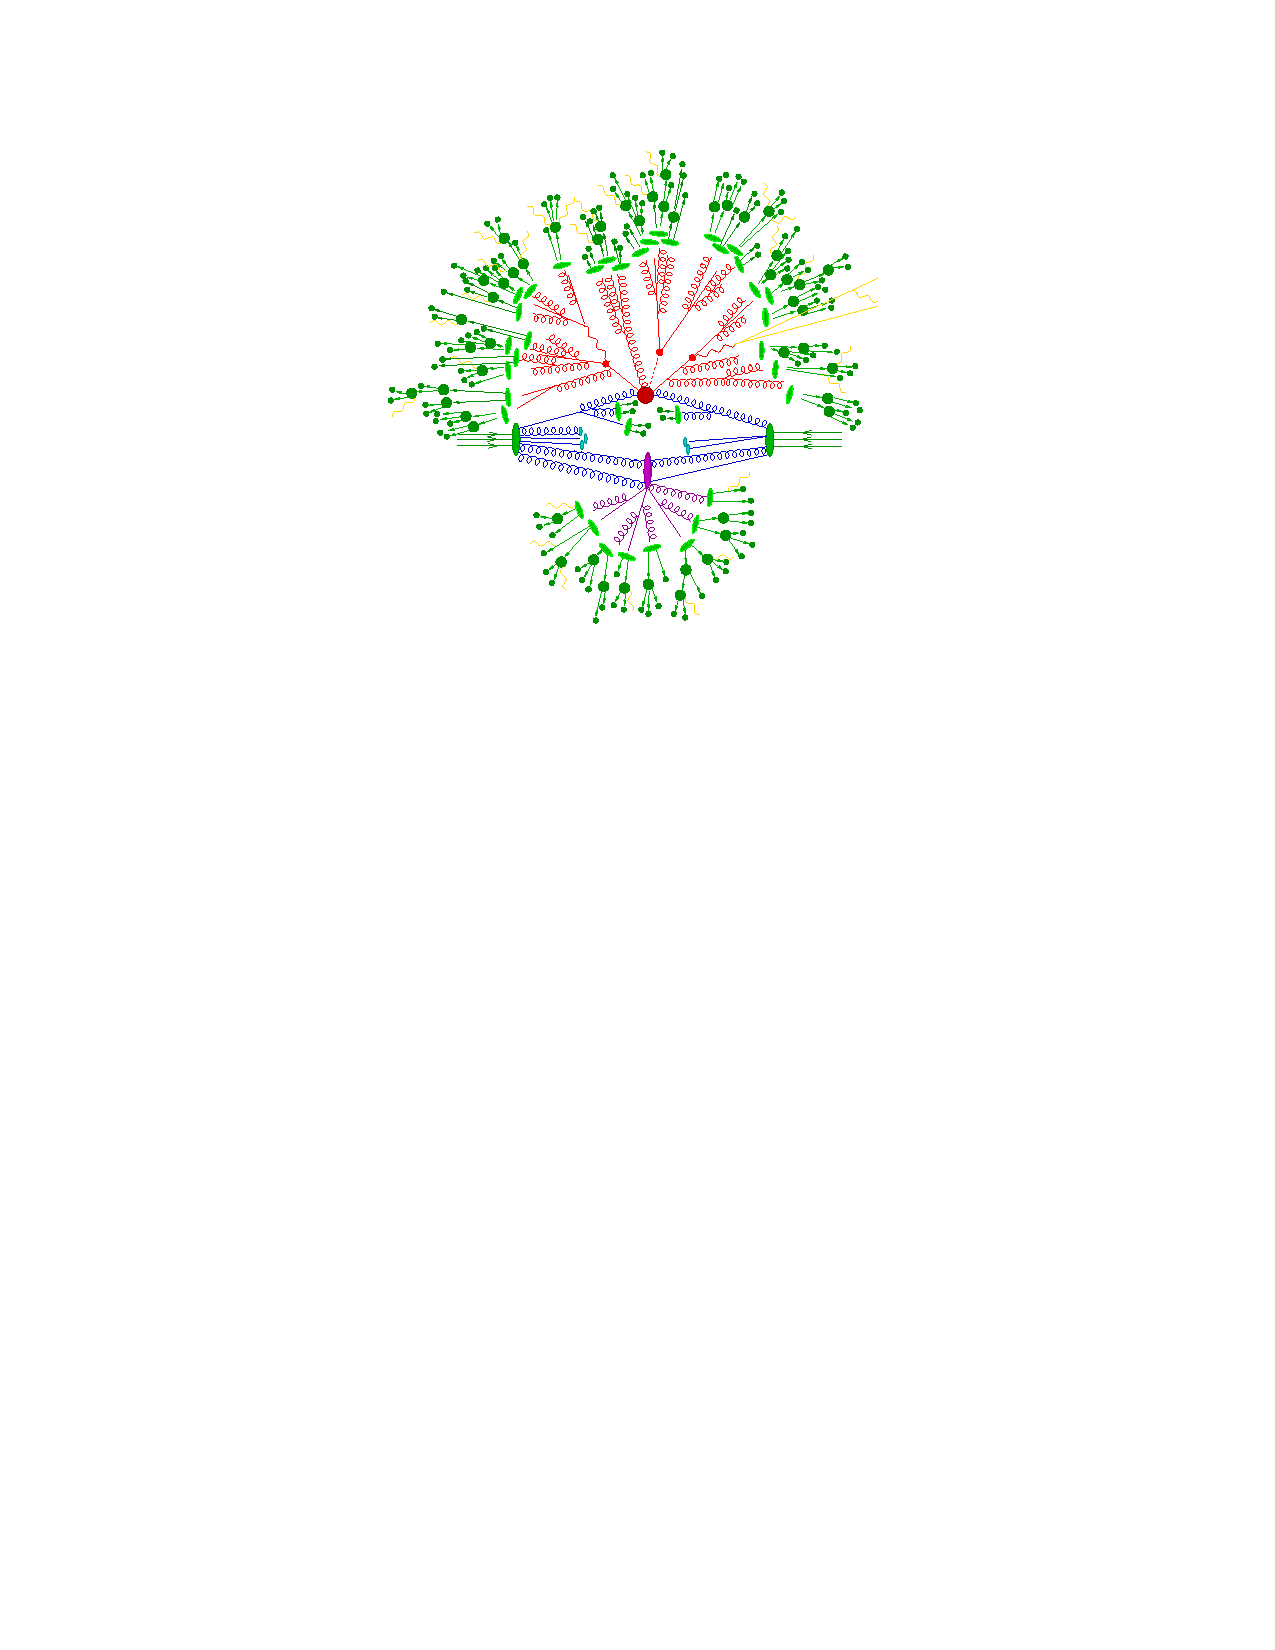
\includegraphics[width=.75\textwidth]{parton-shower}
    \caption{Simulation of an evolution of a proton proton collision: The red circle at the center is the hard collision and the purple oval a secondary hard scatter event. Both are surrounded by a tree-like structure of \ac{qcd} bremsstrahlung interactions simulated with a parton shower. Light green represent hadrons whereas their subsequent decays are shown in dark green. Photons are depicted in yellow. Adopted from \citep{Hoche:2014rga}.
        \label{fig:parton_shower}}
\end{figure}

In a final step the detector response of simulated final state particles is simulated with \textsc{Geant}4 \citep{Agostinelli:2002hh}. It models the detector geometry, the particle's path through the magnetic fields and the particle interactions with the detector material, potentially producing new particles or decays. The output of this step are energy deposits in the various subdetectors of \ac{atlas}. Subsequently these are passed on to a process known as digitization which models the readout electronics. The result of this is raw data being no different from that read out in the actual experiment.

\section{Analysis strategy}
This section describes the event selection and analysis strategy. A detailed description of reconstructed physical objects is given in chapter \ref{ch:reco}. Events only from a Good Runs List are chosen to avoid events where e.g. the \ac{lhc} beam was not stable and to ensure all detectors  are operating as expected.

\subsection{Trigger}
As outlined in section \ref{sec:tdaq} events need to be preselected. The \ac{hlt} applied in this analysis selects events with a large transverse energy $E_\text{T}$ large-$R$ jet. The definition slightly changed over the data taking years as can be seen in table \ref{tab:trigger}.
\begin{table}[htbp]
    \centering
    \caption{Trigger selections per data taking year and minimum requirements on transverse energy $E_\text{T}$ and mass $m$ on the large R jet. }
    \begin{tabular}{ccc}
        \hline
        Year & $E_\text{T}$ & $m$   \\ \hline
        2015 & $>360$       & 0     \\
        2016 & $>420$       & 0     \\
        2017 & $>420$       & $>35$ \\
        2018 & $>420$       & $>40$ \\ \hline
    \end{tabular}
    \label{tab:trigger}
\end{table}
Previous studies have shown that they become fully efficient at about $\pt>\qty[]{420}{GeV}$ \citep{ATL-COM-PHYS-2020-083,ATL-COM-PHYS-2023-033}.
% Figure \ref{fig:trigger_eff} depicts the efficiencies for the different triggers that become fully efficient at about $\pt>\qty[]{420}{GeV}$.
% \begin{figure}
%     \centering
%     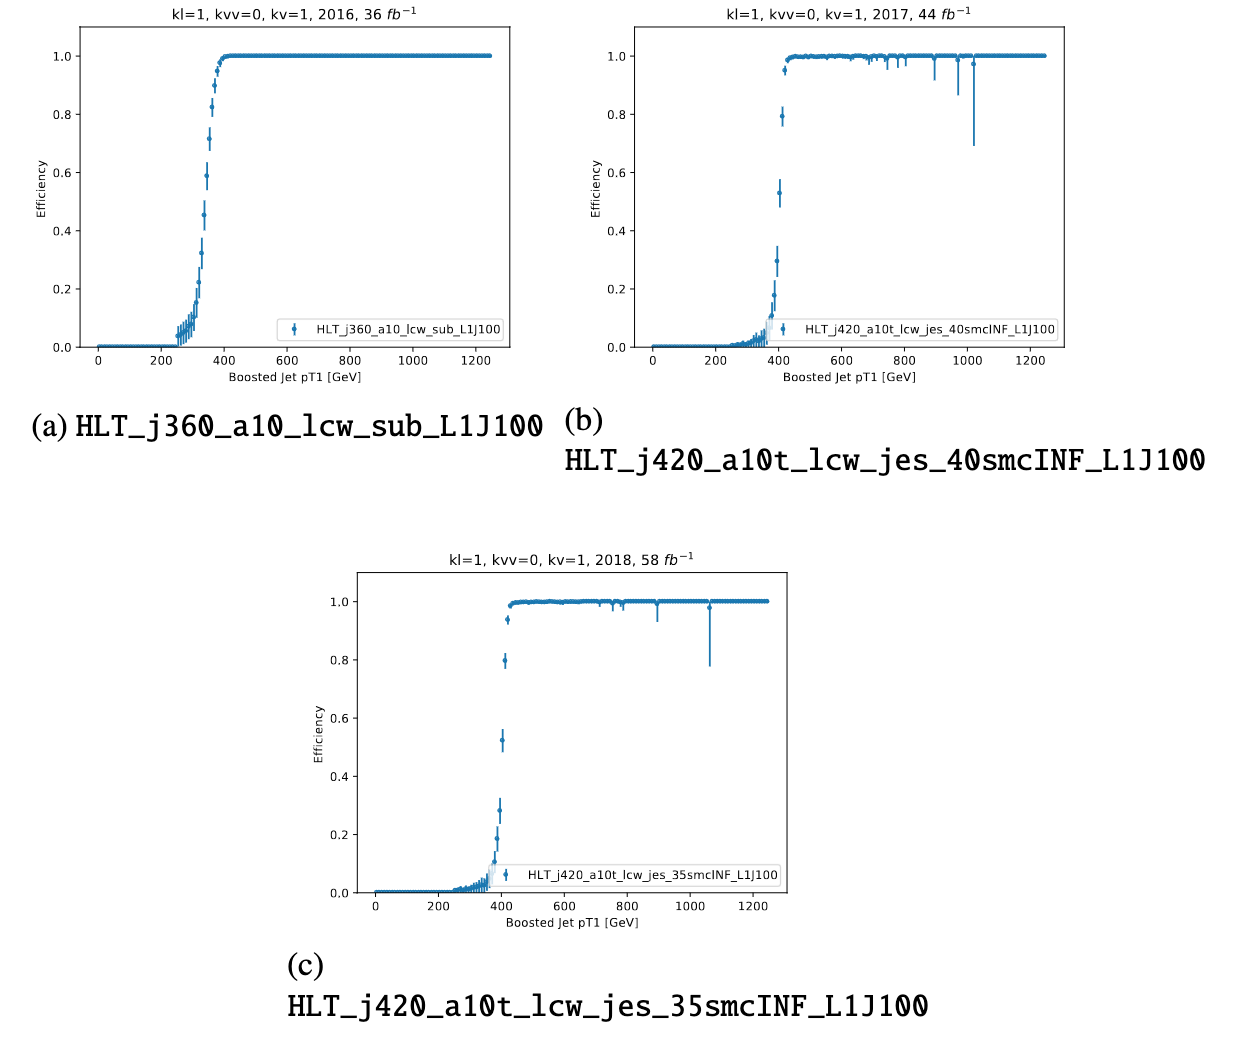
\includegraphics[width=1\textwidth]{trigger_eff}
%     \caption[]{{TODO MYSELF}}
%     \label{fig:trigger_eff}
% \end{figure}

\subsection{Large Radius Jets}
To fully capture the boosted Higgs pair topology two \ac{ufo} large $R=1.0$ jets are selected as described in section \ref{sec:jets}. These enclose the two boosted collimated $b$-jets in each of them to form the Higgs candidates. If there are several large-$R$ jets the two with the highest \pt are chosen. The large-$R$ jets are required to be within $200<p_{\text{T}}<3000$ GeV and $50<m<600$ GeV for which the calibration is valid

\red{$|\eta|<2$, rel 21 did not do this one, even though they are saying it or it is applied somewhere else, because to capture also very boosted? i havent applied it either}.

To be fully efficient on the trigger the leading large-$R$ jet is required to have $\pt>\qty[]{450}{GeV}$. For decay products to be inside a jet approximately $R\approx 2m/\pt$ holds with the mass $m$ and transverse momentum of the parent particle \citep{ATLAS-CONF-2020-022}. For a Higgs mass of \qty[]{125}{GeV} to be contained inside a large-$R$ jet the Higgs candidates therefore must have $\pt\gtrsim \qty[]{250}{GeV}$ and is thus chosen as the \pt requirement on the sub-leading Higgs candidate. If there are several large-$R$ jets the two leading \pt jets are selected. Additionally both Higgs candidates have a mass requirement $m>\qty[]{50}{GeV}$ to reduce \ac{qcd} background. The GN2X tagger described in \ref{sec:gn2x} is used to identify if a selected large-$R$ jet contains two $b$-jets. The top fraction $f_\text{top}(f_\text{Hcc})$ is set to 0.25(0.02) and the \qty[]{60}{\percent} Higgs efficiency \ac{wp} is required with a discriminant depending on the jet mass to avoid mass sculpting as mentioned in \ref{sec:gn2x}.


\subsection{Small Radius Jets}
Two small radius $R=0.4$ jets are required for the \ac{vbf} signature and are referred to as \ac{vbf} jets in the following. They are also reconstructed with the anti-$k_t$ algorithm and as \acp{pfo} as described in \ref{sec:jets}. The tight \ac{wp} for the \ac{jvt} and the LooseBad \ac{wp} for the event cleaning are applied both described in \ref{sec:calibration}. Small-$R$ jets $j$ are selected for $\pt>\qty[]{20}{GeV}$ and $|\eta|<4.5$ and are required to be outside of the Higgs candidate large-$R$ jets $J$ by imposing $\Delta R(J,j) > 1.4$. \red{Further cuts applied on the \ac{vbf} jet system optimized on significance are $|\Delta\eta(j,j)| > 3$ and $m_{jj} > \qty{1}{TeV}$. does neos actually go to zero on mjj}

\subsection{Kinematic Regions}\label{sec:kinematic_regions}
\ac{sr}, Validation Region (VR) and \ac{cr} are explored and optimized in previous analyses \citep{aad2023search,ATL-COM-PHYS-2023-033} in the $m_{H1},m_{H2}$ plane and are defined as
\begin{equation}
    SR=X_{hh} =  \sqrt{\left(\frac{m_{H1} - \SI{124}{\GeV}}{1500 / m_{H1}}\right)^{2} + \left(\frac{m_{H2} - \SI{117}{\GeV}}{1900 / m_{H2}}\right)^{2}} < 1.6,
\end{equation}
\begin{equation}
    \label{VR_Xhh}
    VR =  \sqrt{\left(\frac{m_{H1} - \SI{124}{\GeV}}{0.1 \ln(m_{H1}/\text{GeV})}\right)^{2} + \left(\frac{m_{H2} - \SI{117}{\GeV}}{0.1 \ln(m_{H2}/\text{GeV})}\right)^{2}} < 100,
\end{equation}
and
\begin{equation}
    \label{CR_Xhh}
    CR = \sqrt{\left(\frac{m_{H1} - \SI{124}{\GeV}}{0.1 \ln(m_{H1}/\text{GeV})}\right)^{2} + \left(\frac{m_{H2} - \SI{117}{\GeV}}{0.1 \ln(m_{H2}/\text{GeV})}\right)^{2}} > 100  \ \& \ < 170.
\end{equation}
Figure \ref{fig:m_hh_plane} depicts $m_{H1},m_{H2}$ planes for data and signal samples.
\begin{figure}
    \centering
    % 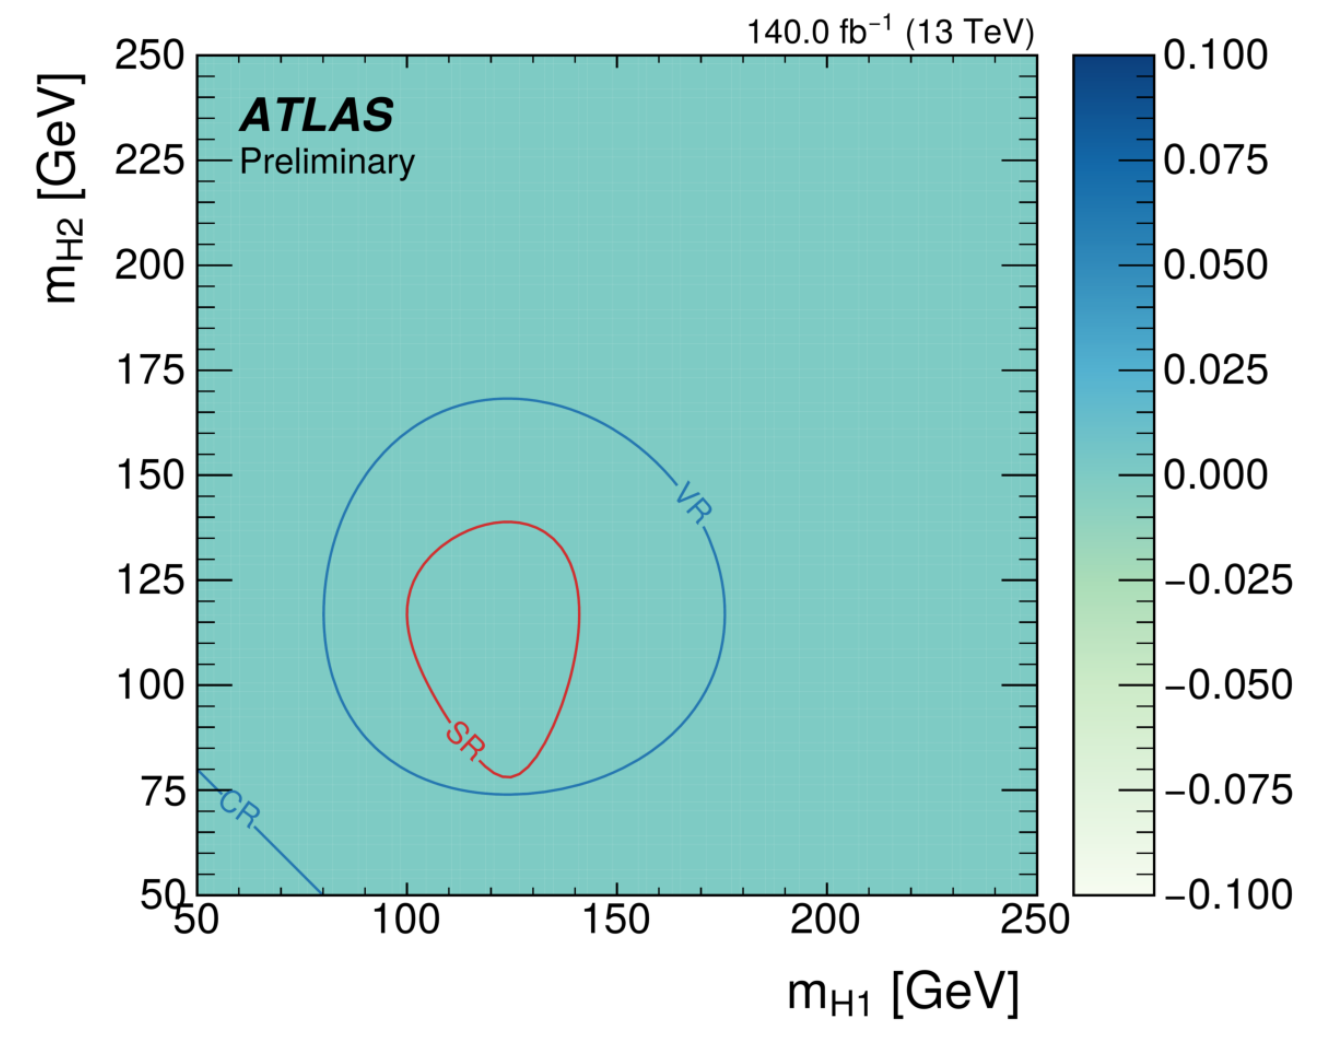
\includegraphics[width=.7\textwidth]{m_hh_plane}
    \subfigure[]{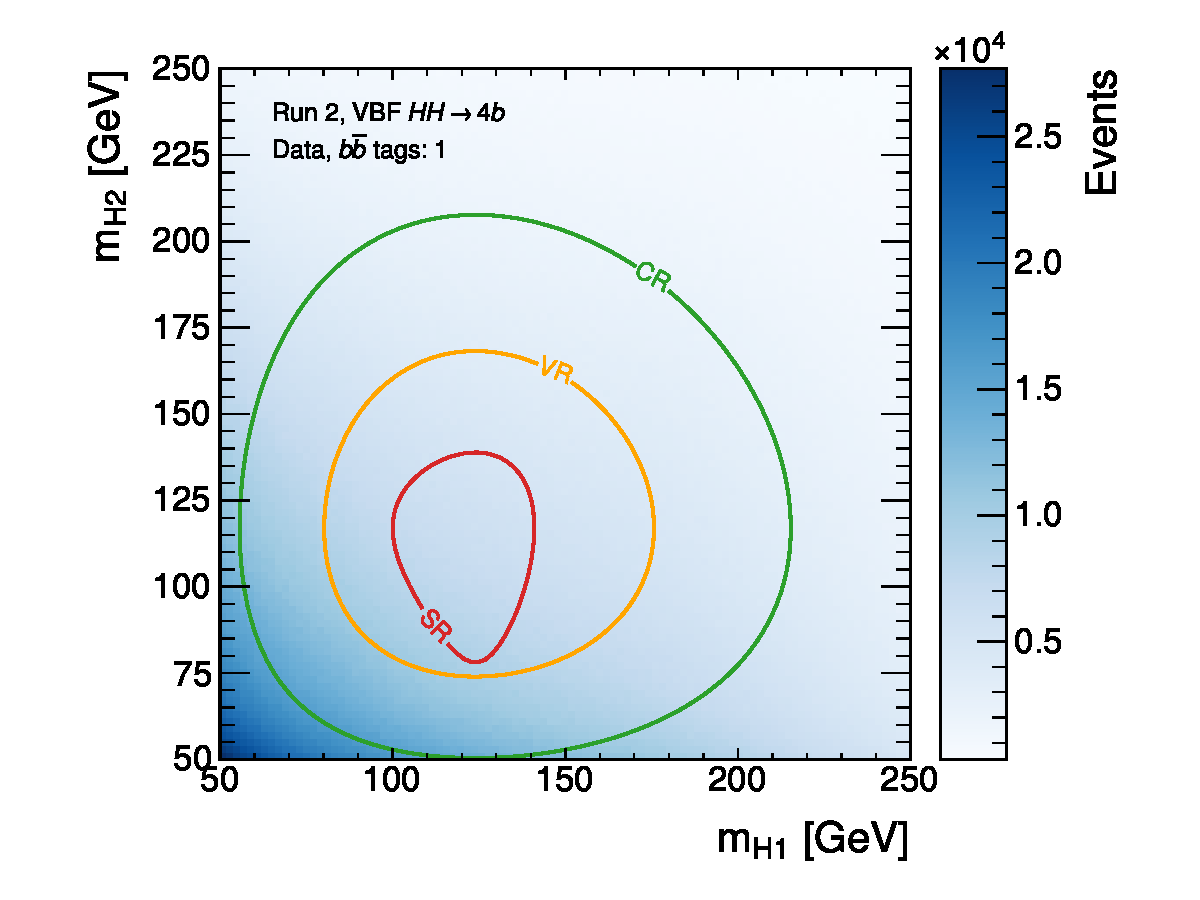
\includegraphics[width=.49\textwidth]{massplane_NOSYS.xbb_1_run2}}
    \subfigure[]{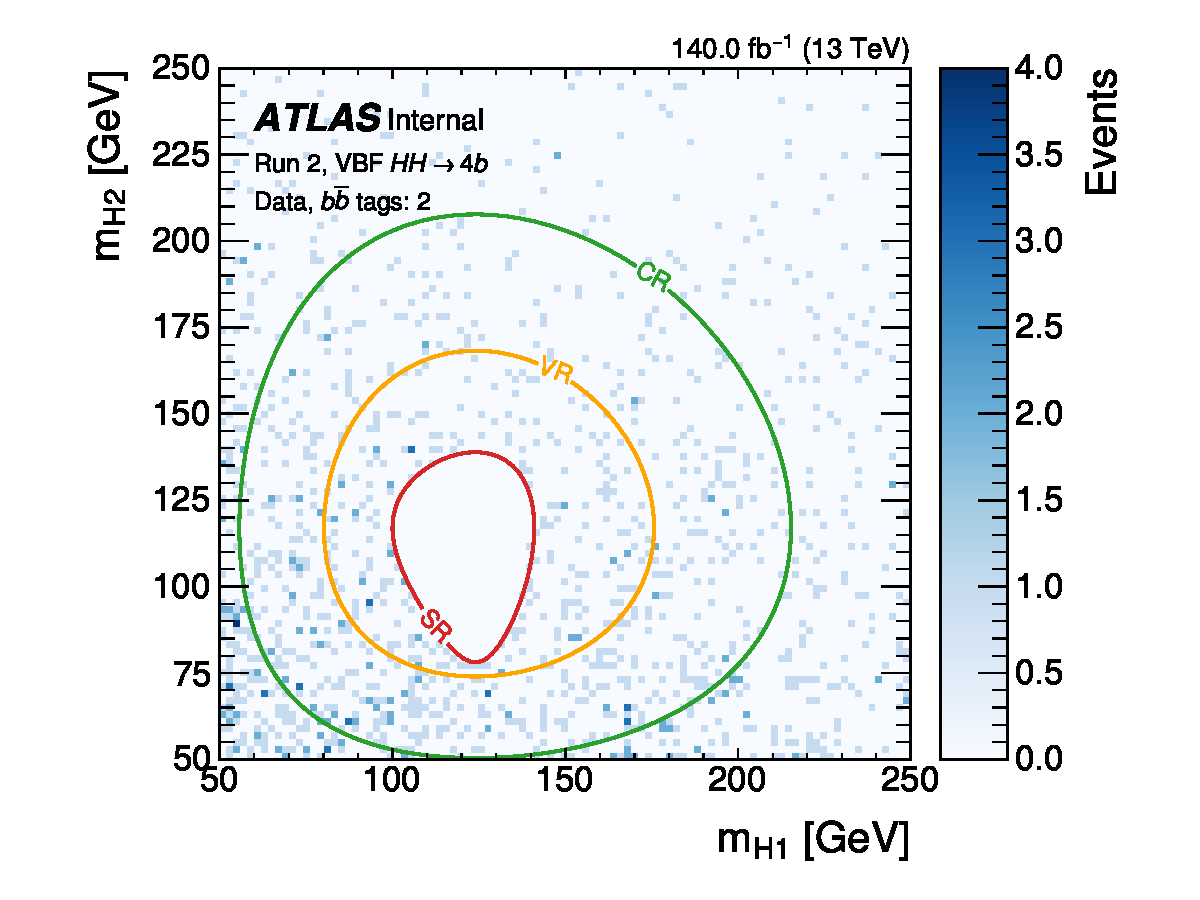
\includegraphics[width=.49\textwidth]{massplane_NOSYS.xbb_2_run2}}
    \subfigure[]{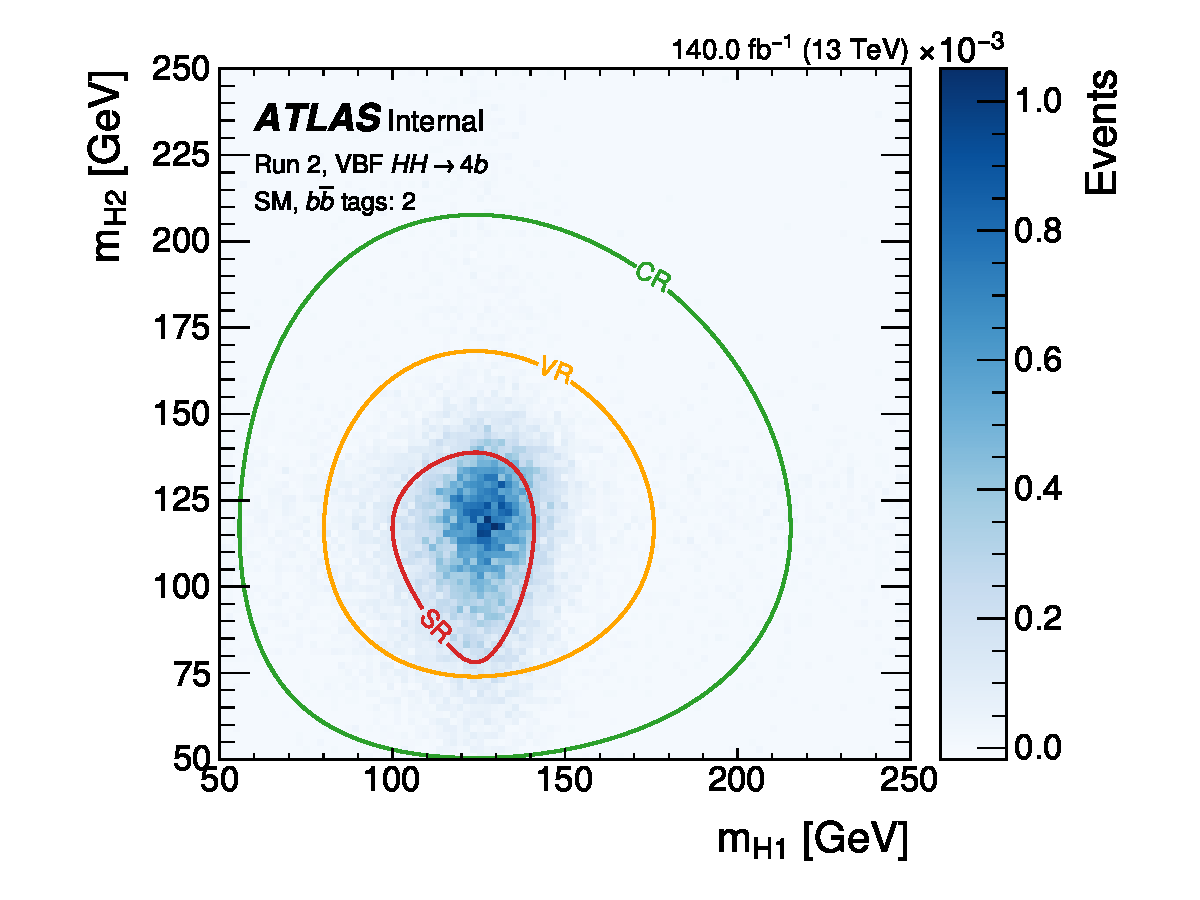
\includegraphics[width=.49\textwidth]{massplane_NOSYS.xbb_2_SM}}
    \subfigure[]{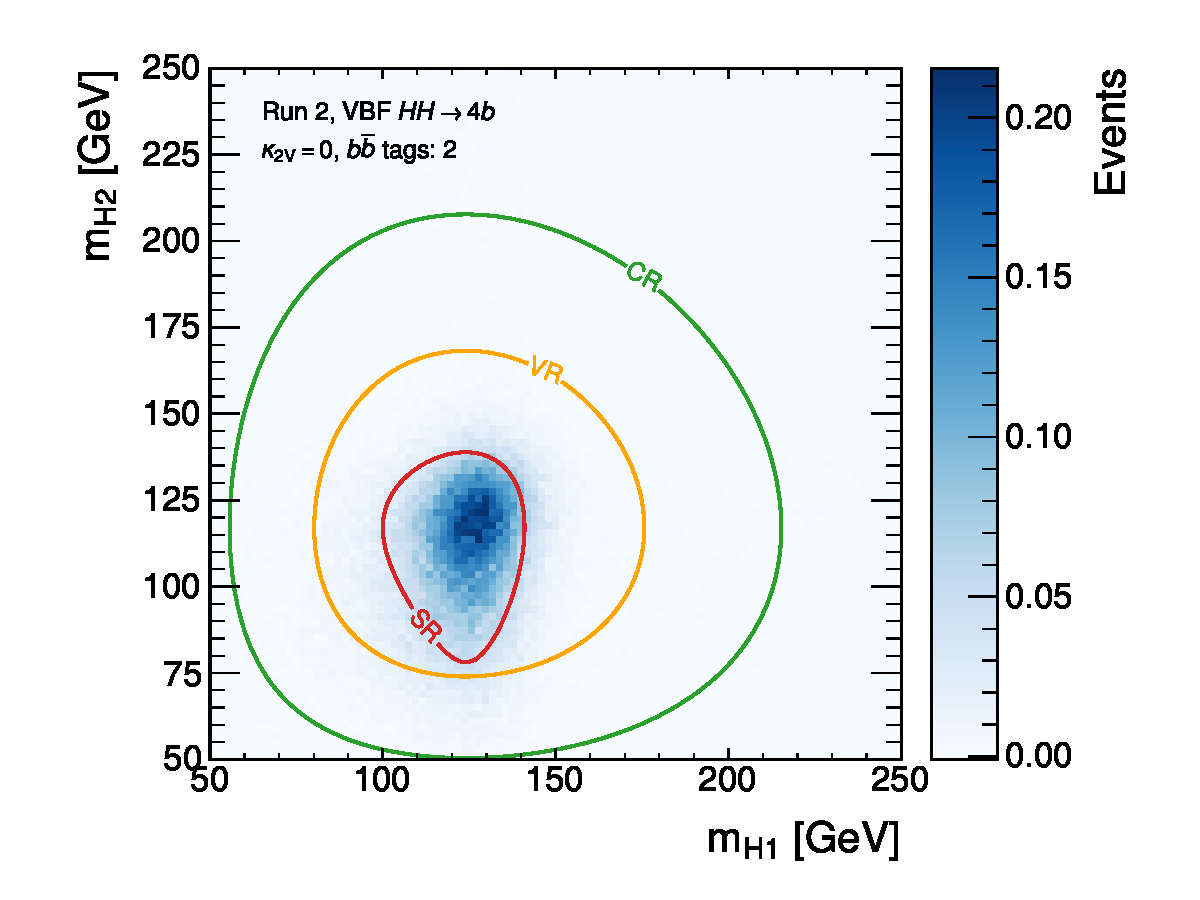
\includegraphics[width=.49\textwidth]{massplane_NOSYS.xbb_2_k2v0}}
    \caption[]{ $m_{H1},m_{H2}$ planes for data with 1 and 2 GN2X tags, a \ac{sm} and $\ktwov$=0 signal sample with 2 GN2X tags. Defined kinematic regions are given as contours for \ac{cr},\ac{vr} and \ac{sr}.}
    \label{fig:m_hh_plane}
\end{figure}

\subsection{Background Estimation}\label{sec:abcd}
Since the final state of this analysis is hadronic it remains a challenging task to estimate the contributions from the plethora of \ac{qcd} processes that contribute to backgrounds via  misidentification of light quarks as heavy $(b, t)$-quarks. Therefore the well established ABCD method is employed to derive a data-driven background estimate \citep{buttinger2018background,PhysRevD.103.035021}. It is based on the idea to use two independent variables e.g. $f$ and $g$ to define four orthogonal regions A, B, C and D as illustrated in figure \ref{fig:abcd} so that for some combination of the ratio of the event yields in the regions hold
\begin{equation}
    \frac{N_A}{N_B}=\frac{N_C}{N_D}.
\end{equation}
\begin{figure}
    \centering
    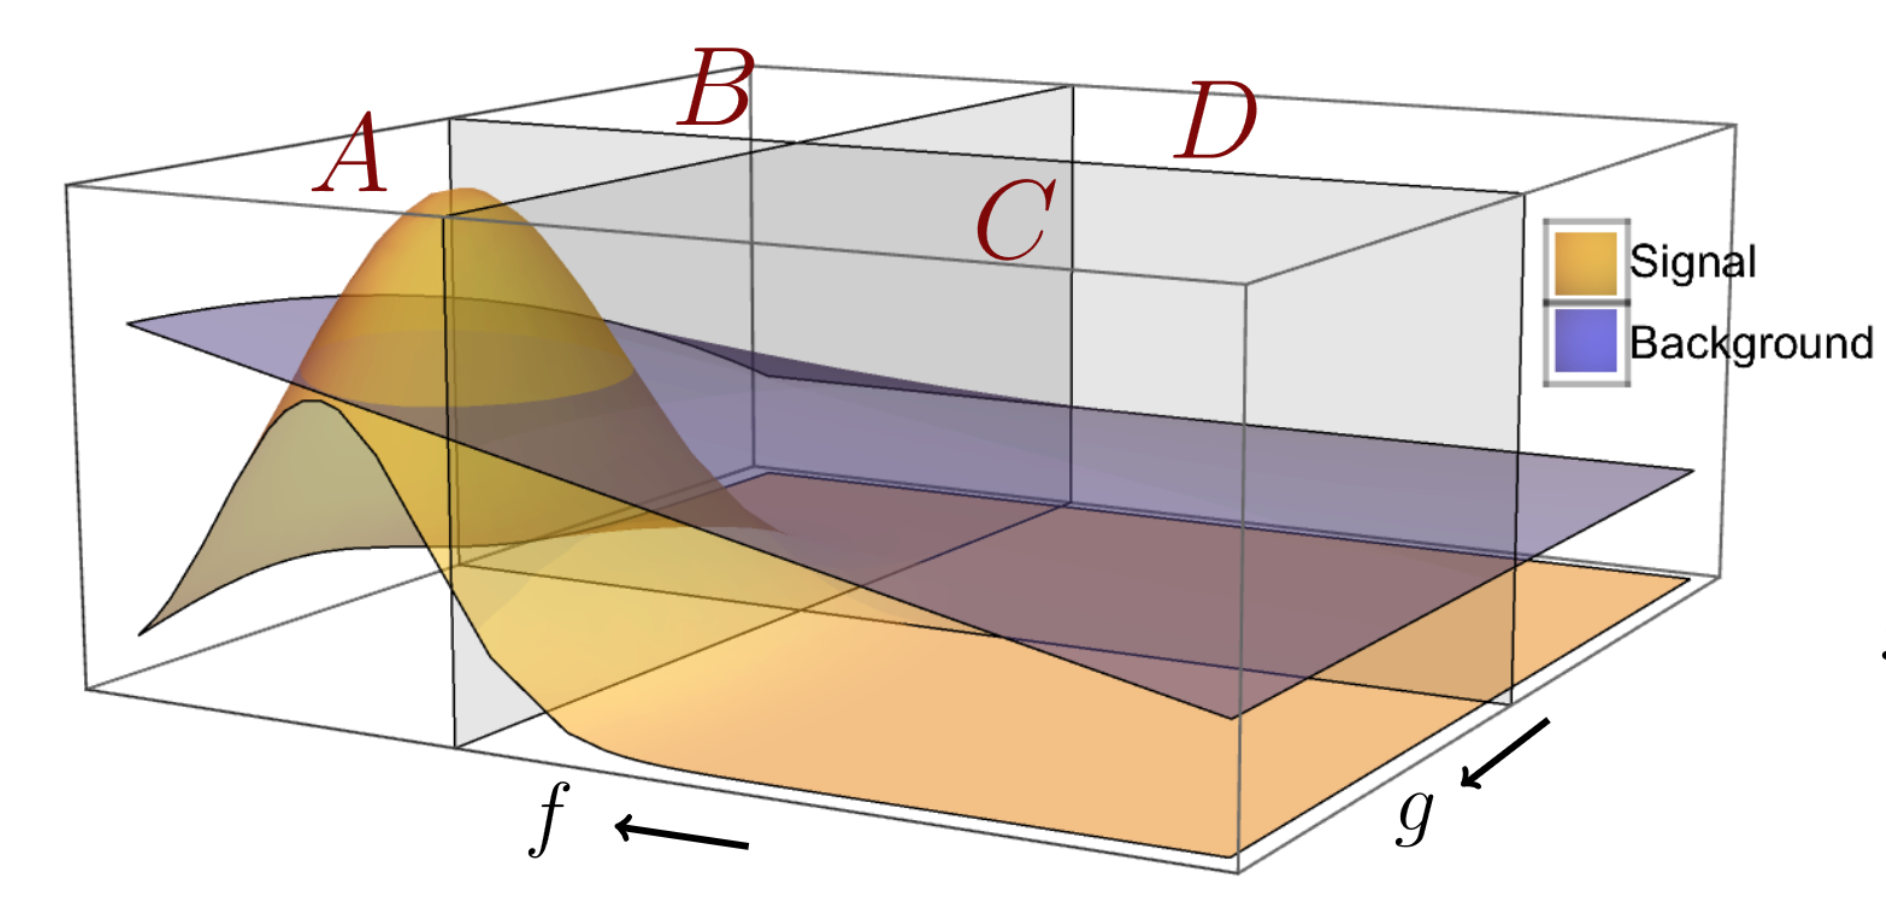
\includegraphics[width=.7\textwidth]{abcd}
    \caption[]{Illustration of four orthogonal regions A,B,C and D defined by two variables $f$ and $g$ in the horizontal and signal and background yields in the vertical dimension. Adopted from \citep{PhysRevD.103.035021}.}
    \label{fig:abcd}
\end{figure}
By rearranging the equation for the unknown $N_A$ an estimate for the background of the signal region can be derived from the other known quantities that lie in the regions dominated by the background. This approach relies on the assumption that the shape of the background in figure \ref{fig:abcd} does not vary greatly between C to D and A to B. Therefore the method must always be tested in a different region to determine its reliability.


In this analysis the two orthogonal variables are defined via the amount of $X\rightarrow bb$ Higgs tagged large-$R$ jets denoted as Xbb and the kinematic regions of the \ac{sr} and \ac{cr} defined in \ref{sec:kinematic_regions}.
\begin{table}[htbp]
    \centering
    \caption{Four orthogonal region definitions for the ABCD method}
    \begin{tabular}{|c|c|}
        \hline
        2 Xbb in CR & 2 Xbb in SR \\ \hline
        1 Xbb in CR & 1 Xbb in SR \\ \hline
    \end{tabular}
    \label{tab:abcd}
\end{table}
This gives the four orthogonal regions shown in table \ref{tab:abcd}. Hence, the background in the \ac{sr} is estimated with a weight extracted from the \ac{cr}
\begin{equation}
    N_\text{SR}^\text{2Xbb}=\frac{N_\text{CR}^\text{2Xbb}}{N_\text{CR}^\text{1Xbb}} N_\text{SR}^\text{1Xbb} = w_\text{CR} N_\text{SR}^\text{1Xbb}=  \red{(0.0039 \pm 0.0002)} \times N_\text{SR}^\text{1Xbb}.
\end{equation}


\subsection{Event Classification}
After the selection of events, a deep feed-forward neural network is employed to construct a histogram suitable for a statistical test of significance. This neural network's training utilizes a novel approach \textsc{neos}, which is thoroughly discussed in Chapter \ref{sec:neos} and optimizes on the $CL_s$ quantity detailed in section \ref{sec:statistics}. Inputs to the neural network include 20 features, which are the four vector components ($\pt,\eta,\phi,m$) of the Higgs boson pair system, the four vector components of the individual Higgs candidates, the two \ac{vbf} jets and the leading score of the GN2X tagger. The \ac{nn} needs to be applicable across all samples, therefore only one GN2X score is incorporated, as the background estimation relies on a single GN2X tag.

The network's architecture features three fully connected layers, each comprising 100 nodes, and concludes with a singular output node. The hidden layers are followed by a rectified linear unit activation function whereas the output node employs a sigmoid activation for classification. The architecture is thus defined as [20,100,100,100,1], indicating the sequence of layers from input to output. Figure \ref{fig:nominal-hist} displays the nominal expected histogram for this analysis

\begin{figure}
    \centering
    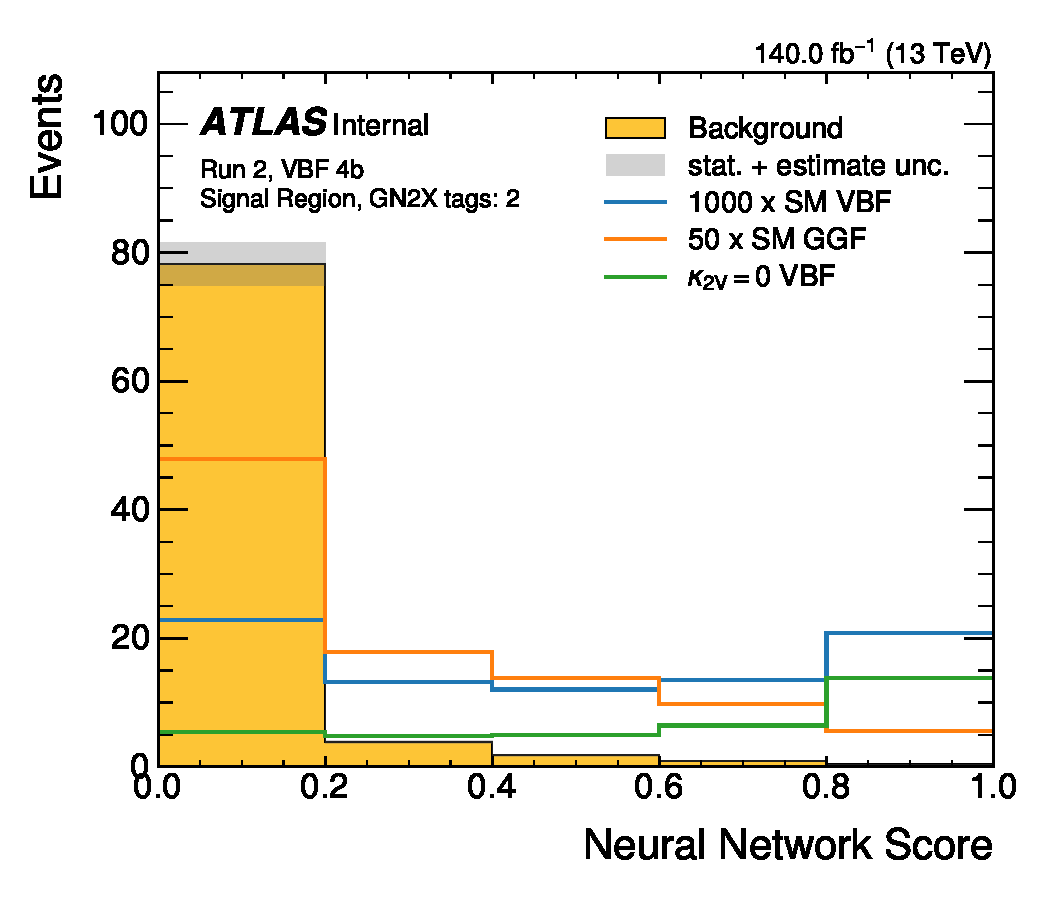
\includegraphics[width=0.7\textwidth]{tomatos_cls_5_NOSYS.SR_xbb_2_nominal_hist.pdf}
    \caption[]{Expected \ac{nn} response to the data-driven background rescaled \ac{sm} signal hypothesis for \ac{vbf} and \ac{ggf} and $\kappa_\text{2V}=0$.}
    \label{fig:nominal-hist}
\end{figure}

\subsection{ABCD method validation}
The ABCD method is validated in the \ac{vr} within statistical uncertainties as displayed in figure \ref{fig:bkg-validation}. It is noted that the previous analysis also studied a binned transfer-factor but did not gain any improvement \citep{ATL-COM-PHYS-2023-033}.
\begin{figure}
    \centering
    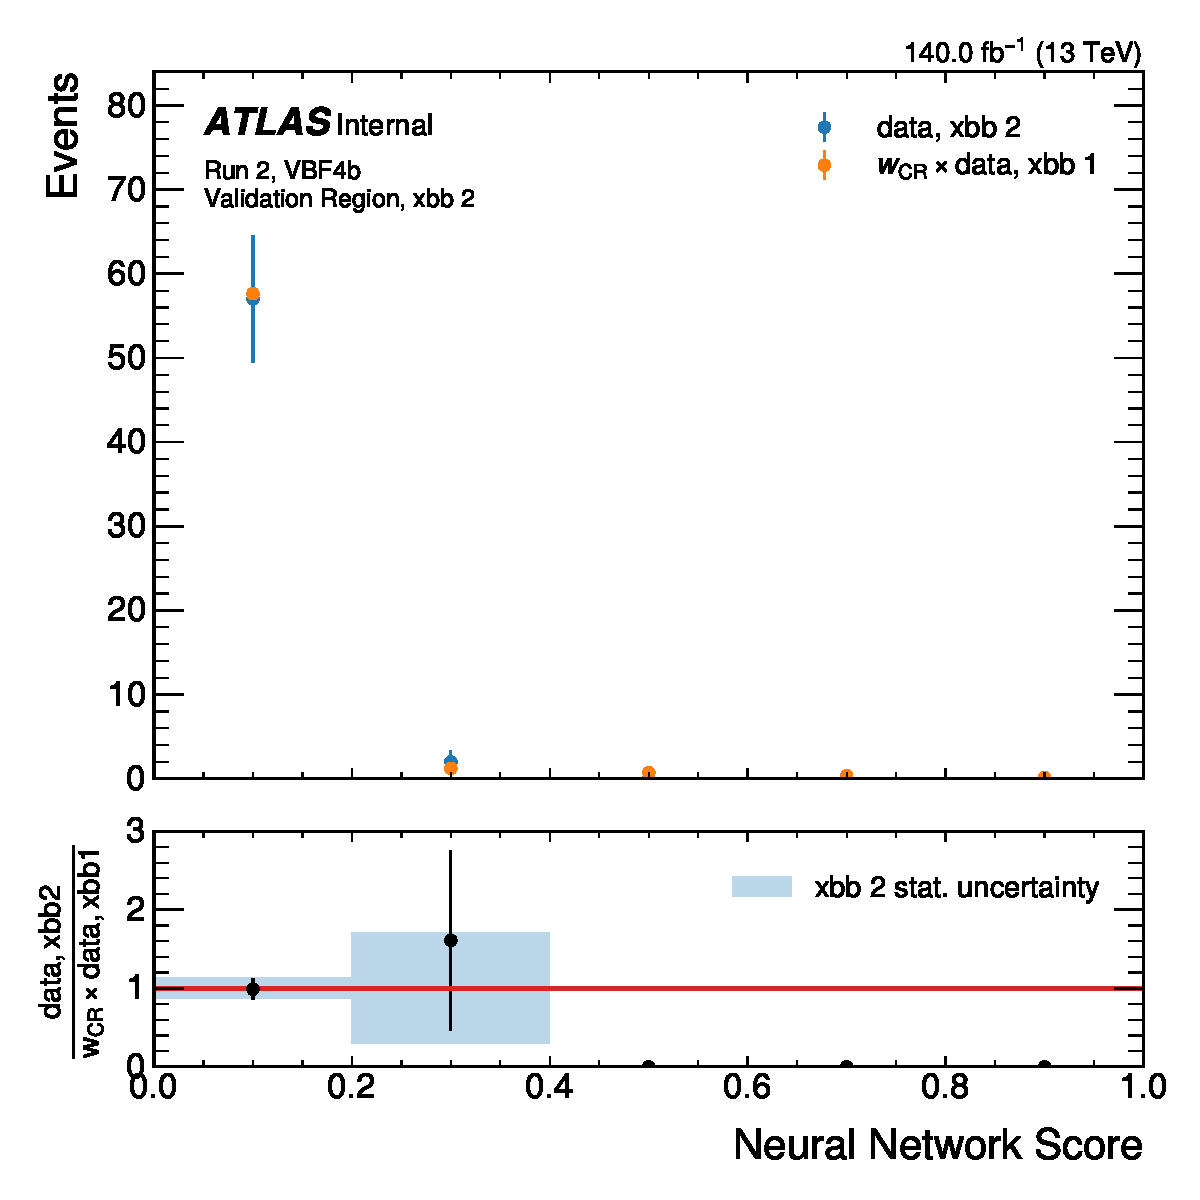
\includegraphics[width=0.7\textwidth]{atos_cls_5_sys_NOSYS.VR_xbb_2_compareABCD}
    \caption[]{The background estimated in the \ac{vr} from data with 1 xbb tag, agrees with data in the \ac{vr} with 2 xbb tags within statistical uncertainties.}
    \label{fig:bkg-validation}
\end{figure}


\section{Linear combination of signal hypotheses}\label{sec:linear_combination}
\newcommand{\kl}{\kappa_\lambda}
\newcommand{\kt}{\kappa_t}
\newcommand{\kvv}{\kappa_\text{2V}}
\newcommand{\kv}{\kappa_\text{V}}
\newcommand{\mhh}{m_\text{HH}}

This analysis is interested in constraining the couplings $\kappa_\text{V},\kappa_\lambda,\kappa_\text{2V}$ associated to the \ac{vbf} processes shown in figure \ref{fig:main_production_processes}. As computing resources are limited and MC generation is unfortunately computationally expensive only a few hypothesis are simulated. However by exploiting the properties of the differential cross-sectional calculation, samples of any hypothesized coupling value can be created through linear combination of samples \citep{ATLAS-CONF-2019-049}. Considering the \ac{vbf} diagrams subscripted as (1,2,3) with couplings $\kl$, $\kv$ and \ktwov the differential (per bin) cross-section of a kinematic variable $x$, e.g. the invariant mass of the Higgs pair system can be rewritten as
\begin{align}
    \label{eqn:xsec_vbf}
    \frac{\mathrm{d}\sigma(\kvv, \kv, \kl )}{\mathrm{d} x } = &
    \left| A(\kvv, \kv, \kl ) \right|^2                                                                                               \\
    =                                                         & \left| \kv \kl M_1(x    ) + \kvv M_2(x  ) + \kv^2 M_3(x   ) \right|^2 \\
    =                                                         & \abs{M_1}^2 \kl^2 \kv^2  + 2 \mathcal{R}(M_{1}^* M_{2})  \kvv \kl \kv \\
                                                              & + 2 \mathcal{R}(M_{1}^* M_{3}) \kl \kv^3 + \abs{M_2}^2  \kvv^2        \\
                                                              & + 2 \mathcal{R}(M_{2}^* M_{3}) \kvv \kv^2 + \abs{M_3}^2 \kv^4.
\end{align}
The amplitude prefactors in front of the couplings depend non-trivially on $x$. However
rewritten as
\begin{align}\label{eq:reweight}
    \frac{\mathrm{d}\sigma(\kvv, \kv, \kl )}{\mathrm{d} x}
    = \; & a_1 \kl^2 \kv^2  + 2 a_2 \kvv \kl \kv  + 2 a_3 \kl \kv^3  \\
         & + a_4 \kvv^2     + 2 a_5 \kvv \kv^2 + a_6\kv^4, \nonumber
\end{align}
and six solutions to this equation, a linear system of equations with variables $a_i$ can be solved and thus $\frac{d\sigma(\kl)}{d x}(\kl)$ as a function of ($\kl$, $\kv$ and \ktwov) allows to deduce the cross-section for a desired hypothesis. Table \ref*{tab:vbf_hh_6term_varlist} shows the list of samples used for the derivation.
\begin{table}
    \centering
    \caption{6-Term VBF Combination Sample Variations}
    \label{tab:vbf_hh_6term_varlist}
    \begin{tabular}{ |l|l|l| }
        \hline
        \textbf {$\kappa_{2V}$} & \textbf {$\kappa_\lambda$} & \textbf {$\kappa_V$} \\
        \hline
        1                       & 1                          & 1                    \\
        1.5                     & 1                          & 1                    \\
        1                       & 2                          & 1                    \\
        1                       & 10                         & 1                    \\
        1                       & 1                          & 0.5                  \\
        1                       & -5                         & 0.5                  \\
        \hline
    \end{tabular}
\end{table}
The approach is employed bin-wise as the extraction factors deviate substantially per bin as shown in figure \ref{fig:linear_combine_bin_solutions}.
\begin{figure}
    \centering
    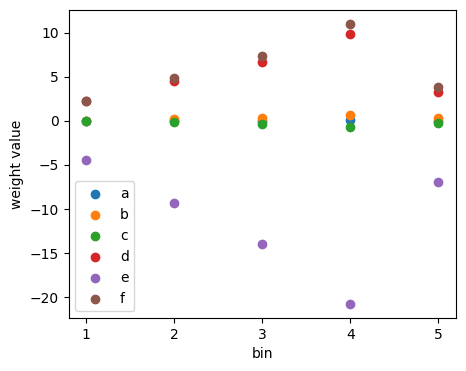
\includegraphics[width=.47\textwidth]{linear_combine_bin_solutions}
    \caption[]{Extracted reweighting factors per bin for equation \ref{eq:reweight}.}
    \label{fig:linear_combine_bin_solutions}
\end{figure}
The method is validated with a mc generated $\ktwov=0$ samples. Figure \ref{fig:tomatos_cls_5_nominal_reweighted_ratio} reveals a \qty[]{5}{\percent} deviation for this approach. \red{should one introduce a very conservative shape uncertainty because of that? the behavior across all values however is unclear with just one validation sample, maybe something for the outlook.}
\begin{figure}
    \centering
    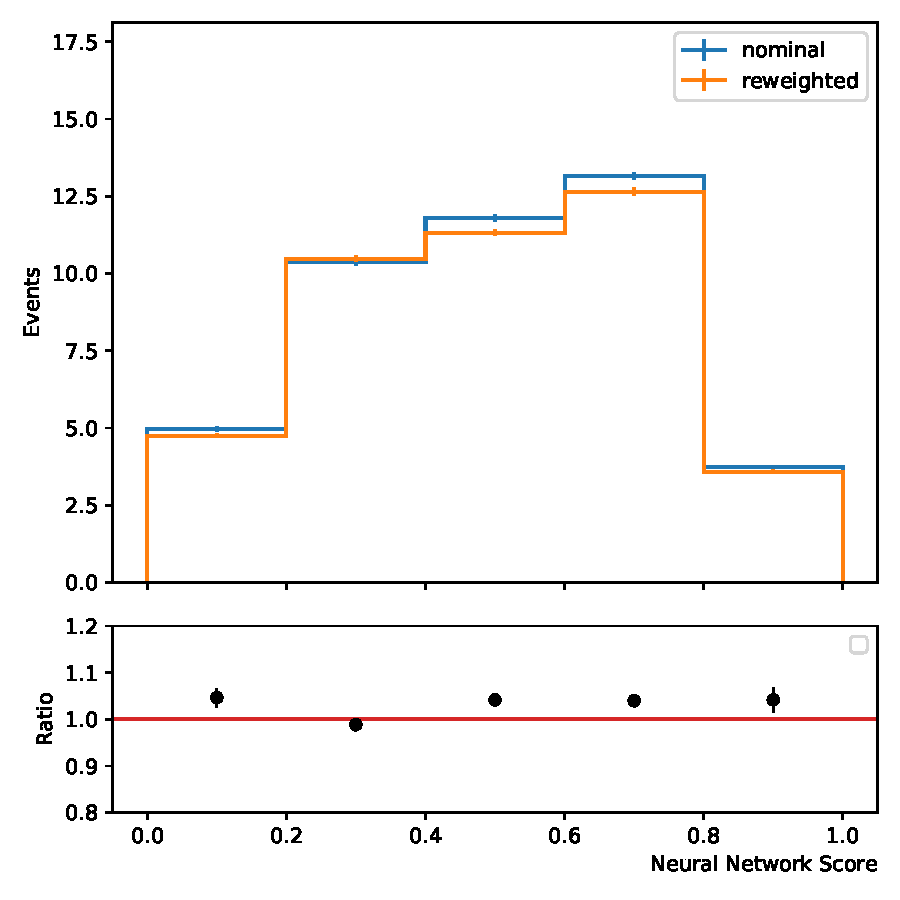
\includegraphics[width=.6\textwidth]{tomatos_cls_5_nominal_reweighted_ratio}
    \caption[]{Comparison between a \ac{mc}-generated $\ktwov=0$ signal sample and a signal sample created with the reweighting approach by linearly combining different \ktwov hypotheses. \red{whats with the mc stat error in general for the reweighted, makes stat err small as taken and scaled in my code from k2v=0}}
    \label{fig:tomatos_cls_5_nominal_reweighted_ratio}
\end{figure}


% , another one would be 
% l0cvv1cv1, however why validating for kl if we scan k2v, I don't think this validation is worth anything in a phase space we are not testing on.



% https://www.overleaf.com/project/638e1930f926cd21d5264259
% https://trexfitter-docs.web.cern.ch/trexfitter-docs/model_building/expression/
% https://gitlab.cern.ch/hh4b/hh4b-boosted-vbf-limits/-/blob/main/create_workspaces/configs/k2V_parameterized_BDT_decorXbb.config?ref_type=heads#L285-331

